\documentclass[conference]{IEEEtran}
\IEEEoverridecommandlockouts
% The preceding line is only needed to identify funding in the first footnote. If that is unneeded, please comment it out.
\usepackage{cite}
\usepackage{amsmath,amssymb,amsfonts}
\usepackage{algorithmic}
\usepackage{graphicx}
\usepackage{textcomp}
\usepackage{xcolor}
\usepackage{url}
\usepackage[spanish]{babel}
\usepackage[utf8]{inputenc}
\usepackage{graphicx}
\usepackage{caption}

\def\BibTeX{{\rm B\kern-.05em{\sc i\kern-.025em b}\kern-.08em
    T\kern-.1667em\lower.7ex\hbox{E}\kern-.125emX}}
\begin{document}

\title{Integración de Dos Robots Móviles en Entornos Colaborativos\\}

\author{\IEEEauthorblockN{Peñúñuri-Félix S.}
\IEEEauthorblockA{\textit{Tecnológico de Monterrey} \\
\textit{A00227286@tec.mx A01641803}\\
IMT \\}
\and
\IEEEauthorblockN{{Gracián-Zepeda R.}}
\IEEEauthorblockA{\textit{Tecnológico de Monterrey} \\
\textit{A01641803@tec.mx A01567011}\\
IMT \\}
\and
\IEEEauthorblockN{{Maldonado-Soto L.}}
\IEEEauthorblockA{\textit{Tecnológico de Monterrey} \\
\textit{A01567011@tec.mx}\\
IMT \\}
\and
\IEEEauthorblockN{{Sánchez-Félix G. }}
\IEEEauthorblockA{\textit{Tecnológico de Monterrey} \\
\textit{A01641788@tec.mx}\\
ITC \\}
}

\maketitle

\textbf{\textit{Abstract}--} \textbf{En este trabajo de investigación, se diseñó, implementó y desarrolló un algoritmo como estrategia para la colaboración de dos robots móviles homogéneos en la ejecución de una tarea. El proyecto comenzó con la implementación de un algoritmo de control para gestionar el comportamiento de los robots y asegurar su movimiento a lo largo de una trayectoria determinada. Se diseñó un sistema multi-agente compuesto por tres agentes: dos robots no holonómicos y un software supervisor, que es una computadora central que actúa como maestro.}


\section{Introducción}
Los sistemas ciber-físicos representan una avanzada integración entre procesos físicos y componentes computacionales, permitiendo el monitoreo y control en tiempo real de operaciones complejas. Este enfoque es fundamental en industrias que requieren niveles elevados de automatización, precisión y adaptabilidad. En este contexto, el presente proyecto se enfoca en desarrollar un sistema ciber-físico que incorpora un robot móvil colaborativo para abordar desafíos específicos de navegación y automatización industrial, de acuerdo con los requisitos establecidos por un socio formador en México.

Con el proyecto se plantea desarrollar un algoritmo que permita el trabajo colaborativo de dos robots móviles de arquitectura homogénea en la ejecución de una tarea, empleando sus características físicas, teniendo en cuenta su entorno y los posibles escenarios que se les pueda presentar. 

El sistema propuesto utiliza un robot TurtleBot3 [12], que es controlado de manera remota mediante el uso de ROS2 [11], con algoritmos implementados en MATLAB [10] y python [13]. Equipado con una unidad de medición inercial (IMU) de 9 grados de libertad, el robot proporciona datos precisos sobre su estado inercial, que son transmitidos a través de la nube a la computadora remota para su monitoreo y control en tiempo real. La integración de una cámara permite el mapeo de su entorno, lo que le permite adaptarse a su entorno, y la coordinación de múltiples robots trabajando en formaciones definidas.

Uno de los proyectos más relevantes es el sistema de navegación autónoma multi-robot desarrollado por \textit{A. Smith, B. Johnson, and C. Wang} [5], donde múltiples robots equipados con sensores LiDAR y cámaras trabajan en conjunto para mapear y explorar áreas industriales de forma autónoma. Este proyecto destaca por su enfoque en la fusión sensorial y el uso de algoritmos de SLAM (Simultaneous Localization and Mapping) en tiempo real, lo que permite a los robots colaborar eficientemente sin intervención humana.

Otro estudio notable es el trabajo de \textit{B. Johnson, M. Leem and T. Singh} [6], que implementa un sistema de comunicación basado en ROS2 para coordinar múltiples robots en tareas de ensamblaje. La investigación se enfoca en la sincronización precisa de movimientos entre los robots, lo que se logra mediante un protocolo de comunicación robusto que minimiza la latencia y asegura la coherencia de los datos compartidos.

Además, \textit{C. Wang, H. Li, and K. Zhao} [7] presentan un enfoque innovador en la gestión de la energía y el control distribuido para robots móviles en entornos de fabricación. Su sistema utiliza una red de sensores inalámbricos para monitorear en tiempo real el estado de los robots y su entorno, permitiendo ajustes dinámicos en la velocidad y la trayectoria para optimizar el consumo de energía sin comprometer el rendimiento.

Por otra parte, \textit{R. García, J. López, and M. Fernández} [8] implementaron un controlador PID clásico en robots diferenciales para tareas de seguimiento de trayectorias en entornos industriales. El uso de un controlador PID permitió ajustar los parámetros de control de manera sencilla y eficiente, logrando un seguimiento preciso de las trayectorias predefinidas, incluso en presencia de perturbaciones externas. Este enfoque se destaca por su simplicidad y robustez, lo que lo convierte en una solución práctica para muchas aplicaciones industriales donde se requiere un control estable y confiable.

Otro trabajo relevante es, \textit{A. Martínez, P. Hernández, and L. Pérez} [9], en el cuál exploraron el uso del algoritmo de control Supertwisting para mejorar la estabilidad y el tiempo de respuesta en robots diferenciales que operan en superficies irregulares. El control Super-Twisting, una variante del control en modo deslizante, se utilizó para compensar las no linealidades inherentes al sistema de control diferencial, proporcionando una respuesta más rápida y precisa en comparación con los controladores tradicionales. Este enfoque es particularmente útil en aplicaciones donde los robots deben lidiar con cambios rápidos en el entorno, manteniendo la estabilidad y minimizando el error en la trayectoria.

El sistema propuesto en el presente proyecto se basa en estos estudios previos, pero introduce mejoras clave en la coordinación y control de robots mediante la integración de una unidad de medición inercial (IMU) y una cámara para el mapeo del entorno. Al implementar algoritmos avanzados de control en MATLAB y Python, y utilizar ROS2 para la comunicación en tiempo real, este proyecto busca superar las limitaciones actuales en la colaboración de robots móviles, particularmente en términos de precisión y adaptabilidad en escenarios industriales complejos.

Con el fin de lograr una implementación exitosa de las estrategias y métodos descritos anteriormente, es esencial comprender el modelo cinemático de un robot diferencial. Este modelo proporciona la base para relacionar las velocidades de las ruedas del robot con su movimiento en el espacio, lo que es crucial para la planificación y control de su trayectoria.

A lo largo de este documento, primero exploraremos en la sección \textbf{Modelo Cinemático} las ecuaciones y principios fundamentales que describen el movimiento de un robot diferencial. A continuación, en la sección \textbf{Desarrollo}, se detallará la implementación práctica de estos principios, incluyendo el diseño de leyes de control y la integración de múltiples capas funcionales en el sistema robótico. Finalmente, en la sección \textbf{Conclusiones}, se discutirán los resultados obtenidos y las perspectivas futuras del proyecto, destacando las contribuciones clave y las áreas de mejora para futuros desarrollos.

\section{Modelo Cinemático}

\subsection{Modelos Cinemáticos en Robots Diferenciales}

El modelo cinemático de un robot diferencial describe la relación entre las velocidades de las ruedas y el movimiento del robot en el espacio. Un robot diferencial se compone de dos ruedas montadas en un eje común, con la posibilidad de control independiente de la velocidad de cada rueda. Este modelo se basa en las siguientes ecuaciones:

\begin{equation}
\mathbf{X}
=
\begin{bmatrix}
x\\
y\\
\theta
\end{bmatrix}
\end{equation}

\begin{equation}
\dot{\mathbf{X}} \
=
\begin{bmatrix}
\dot{x} \\
\dot{y} \\
\dot{\theta}
\end{bmatrix}
=
\begin{bmatrix}
v \cos(\theta) \\
v \sin(\theta) \\
w
\end{bmatrix}
\end{equation}
\begin{equation}
v = \frac{v_r+v_l}{2}
\end{equation}
\begin{equation}
w = \frac{v_r-v_l}{2l}
\end{equation}
\begin{figure}[h!]
    \centering
    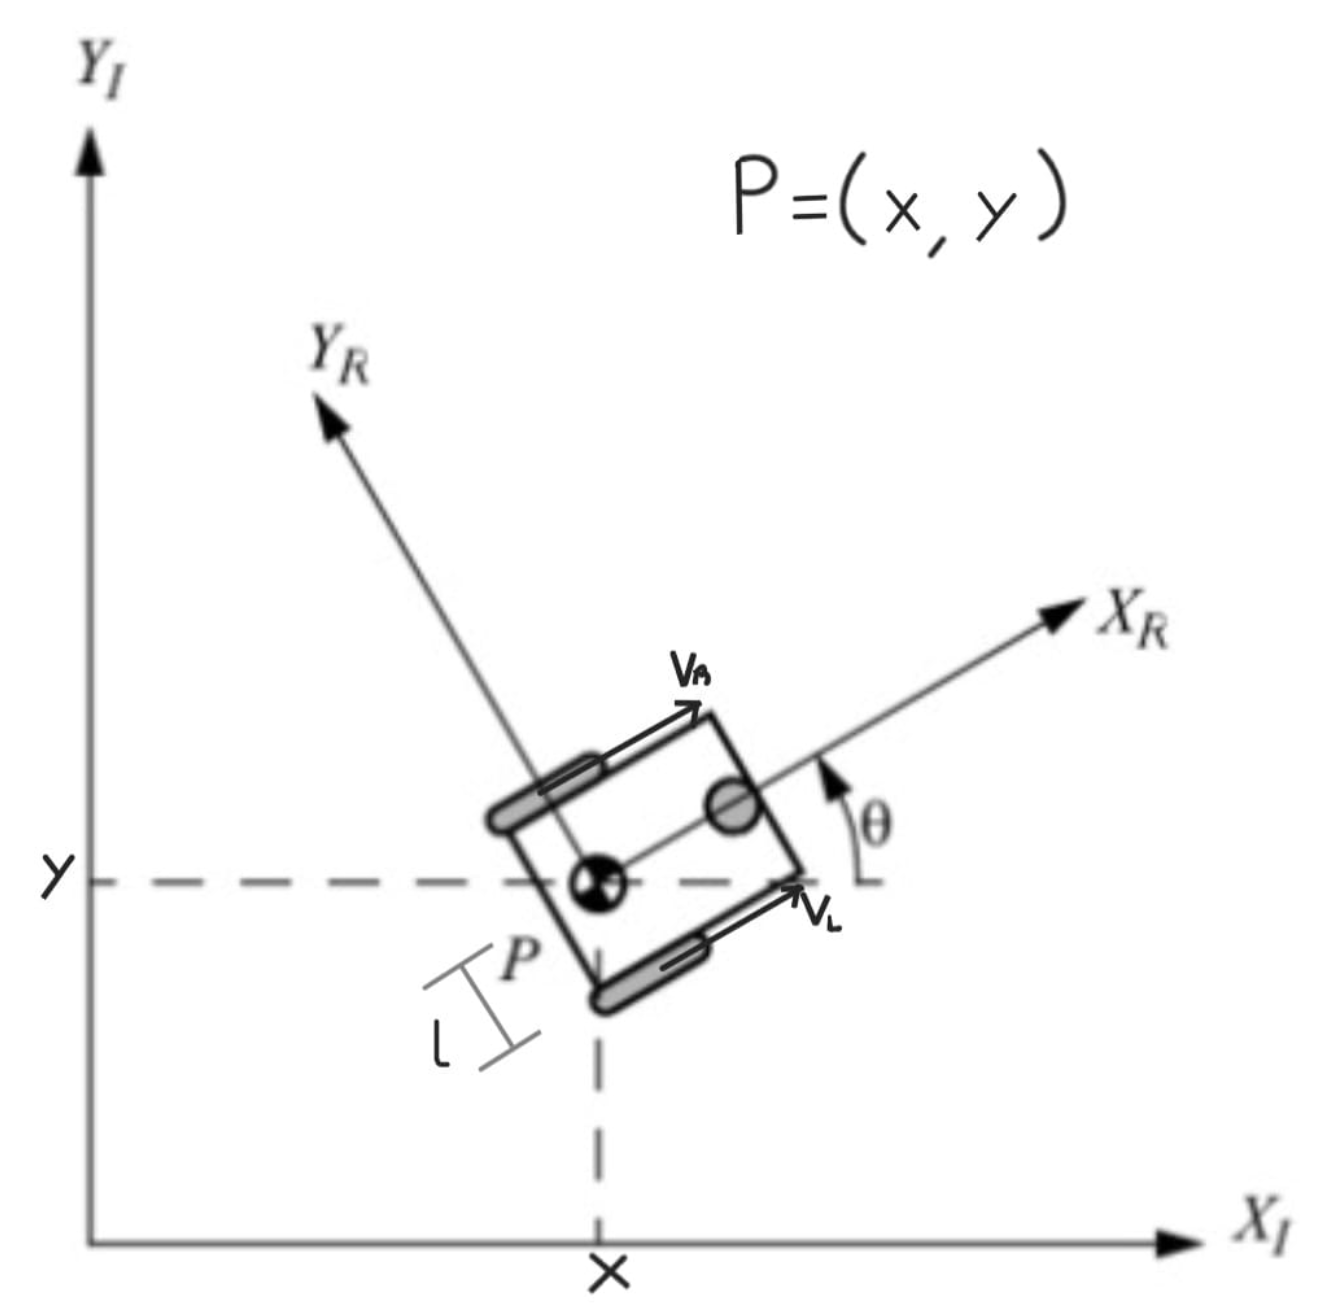
\includegraphics[width=0.5\linewidth]{Robotdiff.png}
    \caption{Robot diferencial}
    \label{fig:imagen de robot diferencial}
\end{figure}

\noindent
donde:
\begin{itemize}
    \item \( \dot{x} \) y \( \dot{y} \) representan las velocidades lineales del robot en las direcciones \(x\) y \(y\), respectivamente.
    \item \( v \) es la velocidad lineal del centro del robot.
    \item \( \theta \) es el ángulo de orientación del robot respecto a un sistema de coordenadas fijo.
    \item \( \dot{\theta} \) es la velocidad angular del robot, es decir, la tasa de cambio de \( \theta \).
    \item \( w \) es la velocidad angular del robot, que se determina a partir de la diferencia en las velocidades de las ruedas.
    \item \( v_r \) es la velocidad de la rueda derecha del robot.
    \item \( v_l \) es la velocidad de la rueda izquierda del robot.
    \item \( l \) es la distancia entre las dos ruedas (ancho del eje).
\end{itemize}

Estas ecuaciones son fundamentales para diseñar los controladores que permiten al robot seguir trayectorias deseadas con precisión. Comprender y aplicar estas ecuaciones es esencial para desarrollar leyes de control efectivas que ajusten las velocidades de las ruedas, asegurando que el robot pueda cumplir con su trayectoria planificada.

\subsection{Ley de Control para Robots Diferenciales}

El control de un robot diferencial se basa en la implementación de leyes de control que permiten ajustar las velocidades de las ruedas para que el robot siga una trayectoria predefinida. Estas leyes de control aseguran la estabilidad del sistema, permitiendo que el robot mantenga un movimiento preciso y controlado. Para que dichas leyes se apliquen de manera efectiva, es fundamental calcular las referencias que guiarán el movimiento del robot en tiempo real.

\subsubsection{Cálculo de Referencias}

El primer paso en este proceso es calcular el ángulo deseado \(\theta_d\) utilizando la función \( \text{atan2} \), lo que permite determinar el ángulo hacia el punto objetivo \((x_d, y_d)\) desde la posición actual del robot \((x, y)\):

\begin{equation}
\theta_d = \text{atan2}((y_d-y),(x_d-x))
\end{equation}


\subsubsection{Cálculo de Errores}

Una vez obtenido el ángulo deseado, es crucial calcular los errores de posición y orientación para corregir la trayectoria del robot y asegurar que siga el camino planificado. Los errores de posición \(d\) y de orientación \(\theta_e\) son fundamentales para el control:

\begin{equation}
d = \sqrt{(x-x_d)^2 + (y-y_d)^2}
\end{equation}

\begin{equation}
\theta_e = \theta - \theta_d
\end{equation}
donde:
\begin{itemize}
    \item \( {d} \) representan la distancia entre el punto de referencia del robot y la posición deseada a donde queremos que llegue el robot.
    \end{itemize}

Para asegurar que el error angular \(\theta_e\) esté dentro del rango \(-\pi\) a \(\pi\), se ajusta de la siguiente manera:

\begin{equation}
\text{if } \theta_e > \pi \text{, entonces } \theta_e = \theta_e - 2\pi
\end{equation}

\begin{equation}
\text{elseif } \theta_e < -\pi \text{, entonces } \theta_e = \theta_e + 2\pi
\end{equation}

Este ajuste es necesario para evitar que el robot realice giros innecesariamente grandes al corregir su orientación. Sin este ajuste, el error angular \(\theta_e\) podría superar \(\pi\) o ser menor que \(-\pi\), lo que implicaría que el robot debería girar en sentido contrario para alinearse con el ángulo deseado. Al mantener \(\theta_e\) dentro del rango \(-\pi\) a \(\pi\), se garantiza que el robot siempre gire en la dirección más corta hacia el punto objetivo, optimizando así su eficiencia y precisión en la navegación.



\subsubsection{Leyes de Control}

La ley de control emplea un controlador proporcional para calcular la velocidad lineal v y la velocidad angular w:

\begin{equation} v = k_{pd} \cdot d \end{equation}

\begin{equation} w = -k_{pr} \cdot \theta_e \end{equation}

Estas ecuaciones permiten simular el comportamiento del robot mientras sigue una trayectoria, ajustando continuamente su orientación y velocidad para alcanzar el punto objetivo. Este enfoque asegura que el error de seguimiento se reduzca progresivamente, lo que mejora la precisión del control durante la navegación del robot.


\subsection{Navegación Autónoma Basada en Visión para Robots Móviles}

En este proyecto, en el marco de la navegación y control de robots móviles, se emplean algoritmos de visión para procesar imágenes en tiempo real y extraer información relevante que permita al robot tomar decisiones de navegación. Estos algoritmos, combinados con datos provenientes de sensores como cámaras y LIDAR, facilitan la estimación continua de la posición y orientación del robot en el espacio, lo cual es esencial para seguir trayectorias precisas. Además, se realiza una fusión de sensores, integrando la información de múltiples fuentes, como cámaras y sensores inerciales (IMUs), para mejorar la precisión en la estimación de la posición y orientación del robot. Este enfoque asegura que el robot mantenga una trayectoria precisa y confiable durante toda su operación.

Con base en estos conceptos y técnicas de navegación, el siguiente paso en el desarrollo del proyecto es la implementación práctica de estas tecnologías. El objetivo es lograr que dos robots se desplacen simultáneamente y colaboren para cargar un objeto sin que se caiga. Para alcanzar este objetivo, se utilizará una cámara para medir la distancia y planificar la ruta de los robots. La información recopilada será procesada en la nube, y se desarrollará un algoritmo de control para gestionar el movimiento de los robots de manera efectiva.

 

\section{Desarrollo}
    Con lo analizado anteriormente, se busca realizar que dos robots puedan desplazarse de forma simultánea, logrando cargar un objeto entre ellos dos sin que se caiga, para esto se tendrá una cámara para medir la distancia y ver la ruta que seguirán los dos robots, esta informción será procesada en la nube y se buscará diseñar un algoritmo de control para el manejo de los robots.
    El proyecto está estructurado en cuatro capas funcionales que trabajan en conjunto para asegurar un rendimiento óptimo del sistema. La Figura \ref{fig:diagrama} muestra la estructura del proyecto en detalle. La primera capa es la de Software, que incluye herramientas críticas como ROS2, MATLAB R2024a y Python 3.11.7, ejecutándose en un entorno Linux. Estas herramientas permiten controlar y coordinar todos los aspectos del sistema, desde la ejecución de algoritmos de control hasta el manejo de datos provenientes de los sensores.
    La siguiente capa es la de Robot, que integra todo el hardware esencial del TurtleBot, incluyendo sensores como LiDAR, IMU, Encoder y una cámara interna, además de los microcontroladores Raspberry Pi 4 y ESP32. Estos componentes son responsables de la gestión de las señales de control y la comunicación entre los distintos módulos del sistema.
    La Manufactura constituye otra capa crucial, donde un estabilizador tipo Stewart juega un papel vital. Este componente garantiza la estabilidad y precisión de la cámara mientras el robot se desplaza por diversos terrenos, lo que es fundamental para la captura de imágenes claras y precisas.
    Finalmente, la capa de Cloud se encarga del almacenamiento y procesamiento de las imágenes capturadas por la cámara, facilitando así la gestión remota de los datos y la toma de decisiones en tiempo real. Todo el sistema está interconectado de manera que se asegura un flujo continuo de comunicación y energía entre los diferentes dispositivos, lo que permite un funcionamiento integrado y eficiente en entornos industriales complejos.

    Para una visión detallada de la estructura del proyecto, consulte el Apéndice A, donde se presenta la Figura \ref{fig:diagrama}.

    Finalmente, presentamos las conclusiones desarrolladas a partir de la elaboración del proyecto.




\section{Conclusiones}

    En conclusión... (concluye)

\begin{thebibliography}{00}
    \bibitem{b1} Hajer Omrane, Mohamed Slim Masmoudi, and M. Masmoudi, “Fuzzy Logic Based Control for Autonomous Mobile Robot Navigation,” Computational Intelligence and Neuroscience, vol. 2016, pp. 1–10.
    \bibitem{b2} Real-time synchronisation method in multi-robot system. \textit{Multi-Robot}. Available: \url{https://www.proquest.com/openview/f9667c88a27f4fe67a51f9e3c0ed778d/1?pq-origsite=gscholar&cbl=5444811}.
    
    \bibitem{b3} F. G. Zambrano Simulación, integración e implementación de un algoritmo de robótica colaborativa para dos robots móviles de arquitectura homogénea. [online]. Disponible en: \url{ http://hdl.handle.net/10654/17713}.
    \bibitem{b4} L. E. Solaque Guzmán, M. A. Molina Villa, y E. L. Rodríguez Vásquez, «Seguimiento de trayectorias con un robot móvil de configuración diferencial», Ing.USBMed, vol. 5, n.º 1, pp. 26–34, jun. 2014.
    \bibitem{b5} A. Smith, B. Johnson, and C. Wang, ``Autonomous Multi-Robot Navigation System for Industrial Applications,'' \textit{IEEE Transactions on Industrial Electronics}, vol. 67, no. 8, pp. 6453-6462, Aug. 2020.
    \bibitem{b6} B. Johnson, M. Lee, and T. Singh, ``Coordinated Multi-Robot Assembly Using ROS2,'' \textit{IEEE Robotics and Automation Letters}, vol. 4, no. 4, pp. 3385-3392, Oct. 2019.

    \bibitem{b7} C. Wang, H. Li, and K. Zhao, ``Energy-Efficient Distributed Control for Mobile Robots in Manufacturing,'' \textit{IEEE Transactions on Control Systems Technology}, vol. 29, no. 5, pp. 2031-2042, Sep. 2021.

    \bibitem{b8} R. García, J. López, and M. Fernández, "Trajectory Tracking for Differential Drive Robots Using PID Control in Industrial Environments," \textit{IEEE Transactions on Industrial Electronics}, vol. 65, no. 8, pp. 6523-6532, Aug. 2018.

    \bibitem{b9} A. Martínez, P. Hernández, and L. Pérez, "Super-twisting Sliding Mode Control for Robust Trajectory Tracking in Differential Drive Robots," \textit{IEEE/ASME Transactions on Mechatronics}, vol. 24, no. 3, pp. 1121-1131, June 2019.
    
    \bibitem{b10} The MathWorks, Inc. (2022). MATLAB version: 9.13.0 (R2022b). Accessed: January 01, 2023. Available: https://www.mathworks.com

    \bibitem{b11} Macenski, T. Foote, B. Gerkey, C. Lalancette, W. Woodall, “Robot Operating System 2: Design, architecture, and uses in the wild,” Science Robotics vol. 7, May 2022

    \bibitem{b12} “TurtleBot3,” Turtlebot.com, 2024. https://www.turtlebot.com/turtlebot3/ (accessed Aug. 29, 2024).

    \bibitem{b13} Python Software Foundation, "Python: A Programming Language," Python Software Foundation, Python version 3.x, [Online]. Available: https://www.python.org/. [Accessed: Aug. 27, 2024].


\end{thebibliography}


\appendices
\section{Estructura del Proyecto}

\noindent\begin{minipage}{\textwidth}
    \centering
    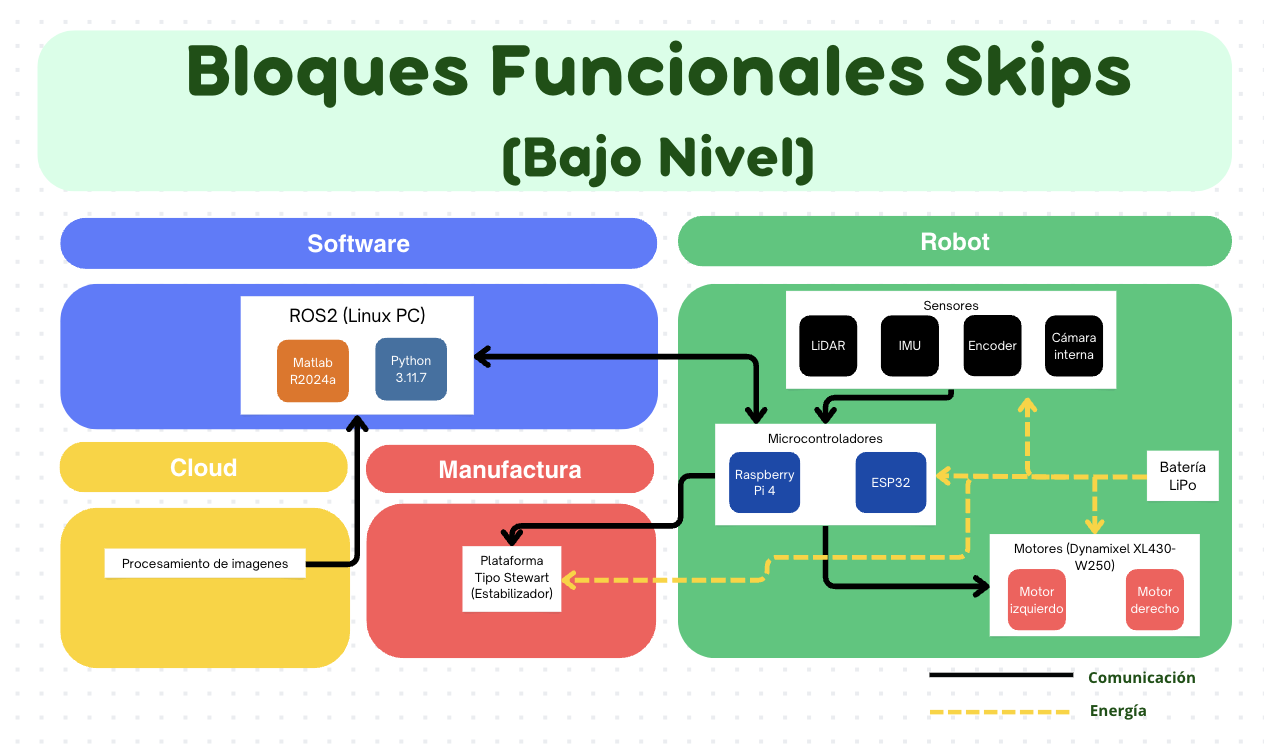
\includegraphics[width=0.95\linewidth]{diagrama.png}
    \captionof{figure}{Estructura del proyecto.}
    \label{fig:diagrama}
\end{minipage}






\vspace{12pt}
\end{document}
